\documentclass[aspectratio=169,11pt]{beamer}

\def\courseTitle{Industrial Security (Master)}
\def\courseSubtitle{Section 02 -- PLC Ladder Logic Reverse Engineering}
\def\sectionNumber{02}
\def\sectionTitle{PLC Ladder Logic Reverse Engineering}

% =====================================================================
% Industrial Security lecture series -- modern Beamer preamble.
%
% Each slide deck must define the following BEFORE \input{}-ing this:
%   \def\courseTitle{...}        e.g. Industrial Security (Bachelor)
%   \def\courseSubtitle{...}     e.g. Section 3 -- Network Architecture
%   \def\sectionNumber{...}      e.g. 03
%   \def\sectionTitle{...}       e.g. Industrial Network Architectures
%
% Optional:
%   \def\courseAuthor{...}       defaults to "Lecture Notes"
%   \def\courseInstitute{...}    defaults to "Department of Computer Science"
%   \def\companyLogo{...}        path to a logo image (PDF/PNG/JPG).
%
% Callout macros (use anywhere inside a frame):
%   \begin{notebox}{title}      ... \end{notebox}
%   \begin{importantbox}{title} ... \end{importantbox}
%   \begin{warningbox}{title}   ... \end{warningbox}
%   \begin{tipbox}{title}       ... \end{tipbox}
%   \begin{defbox}{title}       ... \end{defbox}
%   \begin{takeawaybox}{title}  ... \end{takeawaybox}
%   \begin{quotebox}            ... \end{quotebox}
% =====================================================================

% --- Speaker-notes mode (toggled by Makefile via -usepretex) ----------
% When notesmode=1, build a side-by-side slide+notes PDF for the
% lecturer. When unset/0, build the clean slides-only PDF.
\providecommand{\notesmode}{0}
\ifnum\notesmode=1
  \usepackage{pgfpages}
  \setbeameroption{show notes on second screen=right}
  \setbeamerfont{note page}{size=\small}
\fi

\usepackage[utf8]{inputenc}
\usepackage[T1]{fontenc}
\usepackage[english]{babel}
% Modern type pair: IBM Plex Sans for text, IBM Plex Mono for code.
% Math stays in lmodern; Plex is the dominant family on every text frame.
\usepackage{plex-sans}
\usepackage{plex-mono}
\renewcommand{\familydefault}{\sfdefault}
\usepackage[activate={true,nocompatibility},final,tracking=true,kerning=true,spacing=true,factor=1100,stretch=10,shrink=10]{microtype}
\usepackage{graphicx}
\usepackage{listings}
\usepackage{xcolor}
\usepackage{colortbl}
\usepackage{tikz}
\usepackage{booktabs}
\usepackage{array}
\usepackage{hyperref}
\usepackage{amsmath}
\usepackage{amssymb}
\usepackage{tcolorbox}
\tcbuselibrary{skins, breakable, raster}
\usepackage{fontawesome5}

% =====================================================================
% Shared TikZ styles for the Industrial Security lecture series.
% Loaded by every slide deck and exercise sheet that uses TikZ.
% =====================================================================

\usetikzlibrary{
  arrows.meta,
  shapes,
  shapes.geometric,
  shapes.symbols,
  shapes.multipart,
  positioning,
  fit,
  calc,
  backgrounds,
  decorations.pathmorphing,
  decorations.pathreplacing,
  decorations.text,
  patterns,
  matrix,
  shadows
}

% --- colour palette --------------------------------------------------
\definecolor{isOT}{HTML}{1F4E79}     % OT (deep blue)
\definecolor{isIT}{HTML}{6F2DA8}     % IT (purple)
\definecolor{isSafety}{HTML}{C00000} % safety red
\definecolor{isNet}{HTML}{2E7D32}    % network green
\definecolor{isAttack}{HTML}{B23A48} % attack red
\definecolor{isAccent}{HTML}{E08E0B} % amber
\definecolor{isMute}{HTML}{6B6B6B}   % grey
\definecolor{isLight}{HTML}{EDF2F8}  % light background
\definecolor{isPLC}{HTML}{2C5282}
\definecolor{isHMI}{HTML}{2F855A}
\definecolor{isSCADA}{HTML}{6B46C1}

% --- generic node styles --------------------------------------------
\tikzset{
  isnode/.style={
    draw, rounded corners=2pt, minimum height=8mm, minimum width=18mm,
    font=\small, align=center, thick
  },
  isbox/.style={isnode, fill=isLight},
  plc/.style={isnode, fill=isPLC!15, draw=isPLC, thick},
  hmi/.style={isnode, fill=isHMI!15, draw=isHMI, thick},
  scada/.style={isnode, fill=isSCADA!15, draw=isSCADA, thick},
  sensor/.style={isnode, fill=isNet!10, draw=isNet, minimum height=6mm, minimum width=14mm, font=\scriptsize},
  actuator/.style={isnode, fill=isAccent!15, draw=isAccent, minimum height=6mm, minimum width=14mm, font=\scriptsize},
  firewall/.style={isnode, fill=isAttack!15, draw=isAttack, thick},
  server/.style={isnode, fill=isMute!15, draw=isMute!80, thick},
  switch/.style={isnode, fill=isLight, draw=black!60, minimum height=6mm, minimum width=14mm, font=\scriptsize},
  workstation/.style={isnode, fill=white, draw=isOT, thick},
  attacker/.style={isnode, fill=isAttack!20, draw=isAttack, thick, font=\small\bfseries},
  inetnode/.style={draw, ellipse, minimum width=24mm, minimum height=10mm, font=\scriptsize, fill=isLight, thick},
  process/.style={isnode, fill=isOT!15, draw=isOT, thick, minimum width=24mm},
  zone/.style={
    draw, rounded corners=4pt, thick, dashed, inner sep=4mm
  },
  conduit/.style={-{Stealth[length=2.5mm]}, thick, isNet!80!black},
  attack/.style={-{Stealth[length=2.5mm]}, thick, isAttack, dashed},
  flow/.style={-{Stealth[length=2.5mm]}, thick, isOT!70!black},
  netline/.style={thick, black!60},
  axisline/.style={-{Stealth[length=2mm]}, thick, black!70},
  tag/.style={font=\scriptsize\itshape, fill=white, inner sep=1pt},
  level/.style={
    draw, fill=isLight, minimum width=0.85\linewidth, minimum height=8mm,
    font=\small, anchor=west
  },
  brace/.style={decorate, decoration={brace, amplitude=4pt, raise=2pt}},
  legendbox/.style={draw, rounded corners=2pt, fill=isLight, inner sep=2mm, font=\scriptsize, align=left}
}

% --- handy macros ----------------------------------------------------
% \plcicon, \hmiicon etc as simple labelled boxes; useful inline.
\newcommand{\plcicon}[1][PLC]{\tikz[baseline=-0.6ex]{\node[plc, minimum width=10mm, minimum height=5mm, font=\scriptsize, inner sep=1pt]{#1};}}
\newcommand{\hmiicon}[1][HMI]{\tikz[baseline=-0.6ex]{\node[hmi, minimum width=10mm, minimum height=5mm, font=\scriptsize, inner sep=1pt]{#1};}}
\newcommand{\fwicon}[1][FW]{\tikz[baseline=-0.6ex]{\node[firewall, minimum width=10mm, minimum height=5mm, font=\scriptsize, inner sep=1pt]{#1};}}


\graphicspath{{.}{../../../template/}}

% --- defaults --------------------------------------------------------
\providecommand{\courseAuthor}{Lecture Notes}
\providecommand{\courseInstitute}{Department of Computer Science}
\providecommand{\companyLogo}{logo}

% --- modern palette --------------------------------------------------
\definecolor{slideAccent}{HTML}{1F4E79}       % primary navy
\definecolor{slideSecondary}{HTML}{E08E0B}    % amber accent

% --- Corporate branding overrides ------------------------------------
% A user-editable `branding.tex` at the repo root can override the
% logo path, author/institute lines, and brand colours. If the file is
% missing the built-in defaults above stay in effect.
\IfFileExists{../../../branding.tex}{% =====================================================================
% Corporate / institutional branding -- single file to customise the
% look of the entire course (slides, notes, exercises, labs).
%
% HOW TO REBRAND IN UNDER A MINUTE:
%   1. Replace `branding/logo.pdf` with your own logo
%      (PDF preferred; PNG and JPG also work -- name it `logo.<ext>`).
%   2. (Optional) change the two colours below to your brand palette.
%   3. (Optional) override the author/institute lines below.
%   4. Re-run `make` at the repo root. That's it.
%
% Everything in this file has sensible defaults; you can delete a line
% to fall back to the built-in defaults, or comment it out.
%
% This file is loaded automatically by the slides, exercise, and lab
% preambles -- you never need to \input it manually.
% =====================================================================

% --- Logo --------------------------------------------------------------
% Path is resolved from each leaf-build directory; the default points at
% the shared `branding/` folder at the repo root. If you put your logo
% somewhere else, set the full or relative path here (without extension):
\renewcommand{\companyLogo}{../../../branding/logo}

% --- Author / institute (appears on the title page footer) ------------
\renewcommand{\courseAuthor}{}
\renewcommand{\courseInstitute}{}

% --- Brand colours ----------------------------------------------------
% slideAccent      = primary brand colour (title bands, accent rule)
% slideSecondary   = secondary brand colour (section badge, highlight)
% Both use HTML hex codes. Keep enough contrast against white text.
\definecolor{slideAccent}{HTML}{00205B}      % deep navy
\definecolor{slideSecondary}{HTML}{00A0DC}   % light blue accent
}{}
\definecolor{slideTitle}{HTML}{0F2A44}        % near-black navy
\definecolor{slideMuted}{HTML}{6B6B6B}
\definecolor{slideBg}{HTML}{FFFFFF}
\definecolor{slidePanel}{HTML}{F4F7FB}
\definecolor{slideRule}{HTML}{D6DEE8}

% Callout colours
\definecolor{calNote}{HTML}{1F4E79}
\definecolor{calImportant}{HTML}{B23A48}
\definecolor{calWarning}{HTML}{C77700}
\definecolor{calTip}{HTML}{2E7D32}
\definecolor{calDef}{HTML}{6B46C1}
\definecolor{calTake}{HTML}{0F2A44}

% --- beamer theme ---------------------------------------------------
\useinnertheme{rectangles}
\usefonttheme{professionalfonts}

\setbeamertemplate{navigation symbols}{}
\setbeamertemplate{itemize items}[circle]
\setbeamertemplate{enumerate items}[default]
\setbeamertemplate{section in toc}[ball numbered]
\setbeamercolor{section in toc}{fg=slideTitle}

% Colours
\setbeamercolor{normal text}{fg=slideTitle, bg=slideBg}
\setbeamercolor{title}{fg=slideAccent}
\setbeamercolor{subtitle}{fg=slideMuted}
\setbeamercolor{frametitle}{fg=slideAccent}
\setbeamercolor{structure}{fg=slideAccent}
\setbeamercolor{itemize item}{fg=slideAccent}
\setbeamercolor{itemize subitem}{fg=slideSecondary}
\setbeamercolor{block title}{fg=white, bg=slideAccent}
\setbeamercolor{block body}{fg=slideTitle, bg=slidePanel}
\setbeamercolor{alerted text}{fg=slideSecondary}

% Fonts
\setbeamerfont{title}{series=\bfseries, size=\Large}
\setbeamerfont{subtitle}{series=\mdseries, size=\normalsize}
\setbeamerfont{frametitle}{series=\bfseries, size=\large}
\setbeamerfont{block title}{series=\bfseries, size=\normalsize}
\setbeamerfont{footline}{size=\tiny}

% --- frametitle: title bar + accent underline + section badge -------
% The accent rules are wrapped in a zero-width box so they never
% contribute to the surrounding hbox width (no Overfull warnings).
\setbeamertemplate{frametitle}{%
  \nointerlineskip
  \begin{beamercolorbox}[wd=\paperwidth, ht=2.8ex, dp=1.6ex, leftskip=1.2em, rightskip=1.2em]{frametitle}%
    \usebeamerfont{frametitle}\insertframetitle%
    \hfill
    {\color{slideMuted}\small \sectionNumber}%
  \end{beamercolorbox}%
  \nointerlineskip
  \makebox[0pt][l]{\hspace*{1.2em}\textcolor{slideSecondary}{\rule{2.5em}{1pt}}\textcolor{slideAccent}{\rule{\dimexpr\paperwidth-3.7em\relax}{1pt}}}%
  \par\vskip4pt
}

% --- footer ---------------------------------------------------------
\defbeamertemplate*{footline}{is-footer}{%
  \leavevmode%
  \hbox{%
    \begin{beamercolorbox}[wd=.55\paperwidth, ht=2.4ex, dp=1ex, leftskip=1em]{author in head/foot}%
      {\color{slideMuted}\tiny \courseTitle{} \;\; $\bullet$ \;\; Section \sectionNumber{} -- \sectionTitle}%
    \end{beamercolorbox}%
    \begin{beamercolorbox}[wd=.45\paperwidth, ht=2.4ex, dp=1ex, rightskip=1em]{title in head/foot}%
      \hfill {\color{slideMuted}\tiny \insertframenumber{} / \inserttotalframenumber}%
    \end{beamercolorbox}%
  }%
  \vskip2pt
}

% --- listings -------------------------------------------------------
\definecolor{codebg}{HTML}{F4F7FB}
\definecolor{codekw}{HTML}{0F2A44}
\definecolor{codestr}{HTML}{8B3A3A}
\definecolor{codecom}{HTML}{5A7D54}

\lstset{
    backgroundcolor=\color{codebg},
    basicstyle=\ttfamily\scriptsize\color{slideTitle},
    keywordstyle=\color{codekw}\bfseries,
    stringstyle=\color{codestr},
    commentstyle=\color{codecom}\itshape,
    breaklines=true,
    frame=leftline,
    framerule=2pt,
    rulecolor=\color{slideAccent},
    numbers=left,
    numberstyle=\tiny\color{slideMuted},
    numbersep=8pt,
    showstringspaces=false,
    tabsize=2,
    captionpos=b,
    xleftmargin=0.6em
}

% --- callout boxes --------------------------------------------------
% Shared base style for all callout boxes.
% Subtle drop shadow gives the boxes a hint of elevation without distraction.
\tcbset{
  isCallout/.style={
    enhanced, breakable, sharp corners=northeast,
    arc=2pt, boxrule=0pt,
    leftrule=3pt,
    fonttitle=\bfseries\small,
    coltitle=white,
    fontupper=\small,
    left=2mm, right=2mm, top=1.5mm, bottom=1.5mm,
    drop fuzzy shadow=black!30,
    title={#1}
  }
}

\newtcolorbox{notebox}[1]{
  isCallout={#1},
  colback=calNote!8, colframe=calNote, leftrule=3pt,
  colbacktitle=calNote, attach boxed title to top left={xshift=2mm, yshift=-1.2mm},
  boxed title style={colback=calNote, arc=1pt, boxrule=0pt, left=2mm, right=2mm, top=0.5mm, bottom=0.5mm}
}

\newtcolorbox{importantbox}[1]{
  isCallout={#1},
  colback=calImportant!7, colframe=calImportant, leftrule=4pt,
  colbacktitle=calImportant, attach boxed title to top left={xshift=2mm, yshift=-1.2mm},
  boxed title style={colback=calImportant, arc=1pt, boxrule=0pt, left=2mm, right=2mm, top=0.5mm, bottom=0.5mm}
}

\newtcolorbox{warningbox}[1]{
  isCallout={#1},
  colback=calWarning!10, colframe=calWarning, leftrule=4pt,
  colbacktitle=calWarning, attach boxed title to top left={xshift=2mm, yshift=-1.2mm},
  boxed title style={colback=calWarning, arc=1pt, boxrule=0pt, left=2mm, right=2mm, top=0.5mm, bottom=0.5mm}
}

% Alias warnbox = warningbox, with an optional title (default = "Caution")
\newtcolorbox{warnbox}[1][Caution]{
  isCallout={#1},
  colback=calWarning!10, colframe=calWarning, leftrule=4pt,
  colbacktitle=calWarning, attach boxed title to top left={xshift=2mm, yshift=-1.2mm},
  boxed title style={colback=calWarning, arc=1pt, boxrule=0pt, left=2mm, right=2mm, top=0.5mm, bottom=0.5mm}
}

\newtcolorbox{tipbox}[1]{
  isCallout={#1},
  colback=calTip!8, colframe=calTip, leftrule=3pt,
  colbacktitle=calTip, attach boxed title to top left={xshift=2mm, yshift=-1.2mm},
  boxed title style={colback=calTip, arc=1pt, boxrule=0pt, left=2mm, right=2mm, top=0.5mm, bottom=0.5mm}
}

\newtcolorbox{defbox}[1]{
  isCallout={#1},
  colback=calDef!8, colframe=calDef, leftrule=3pt,
  colbacktitle=calDef, attach boxed title to top left={xshift=2mm, yshift=-1.2mm},
  boxed title style={colback=calDef, arc=1pt, boxrule=0pt, left=2mm, right=2mm, top=0.5mm, bottom=0.5mm}
}

\newtcolorbox{takeawaybox}[1]{
  enhanced, breakable, arc=3pt, boxrule=0pt,
  colback=calTake!7, colframe=calTake,
  toptitle=2mm, bottomtitle=2mm,
  fonttitle=\bfseries\normalsize, coltitle=white,
  colbacktitle=calTake,
  fontupper=\small,
  title={\faStar~Key Takeaway: #1},
  left=3mm, right=3mm, top=2mm, bottom=2mm
}

\newtcolorbox{quotebox}{
  enhanced, breakable, arc=2pt, boxrule=0pt,
  colback=slidePanel, colframe=slideMuted,
  leftrule=3pt, top=2mm, bottom=2mm, left=3mm, right=3mm,
  fontupper=\itshape\small,
}

% Convenience: inline highlight badge
\newcommand{\remembertag}{\tikz[baseline=-0.7ex]\node[fill=calImportant, text=white, font=\scriptsize\bfseries, rounded corners=2pt, inner sep=2pt]{REMEMBER};}
\newcommand{\tldr}{\tikz[baseline=-0.7ex]\node[fill=calTake, text=white, font=\scriptsize\bfseries, rounded corners=2pt, inner sep=2pt]{TL;DR};}

% Source attribution: tiny grey line, anchored bottom-left of the content area
% Usage:  \source{Symantec, \emph{W32.Stuxnet Dossier} v1.4, 2011.}
% Multiple sources:  \source{X.\ Y., 2018; Z, 2020.}
\newcommand{\source}[1]{%
  \par\nointerlineskip\vspace{0.4mm}%
  {\color{slideMuted}\fontsize{5.5}{6.5}\selectfont\textit{Source:} #1\par}%
}

% References slide: aggregate citations + further reading at the end of a section.
% Usage:  \referencesframe{ \item ... \item ... }
% The `frame` environment must be written literally in the deck, so this is a
% macro rather than a wrapper environment (beamer collects the frame body and
% trips over \newenvironment wrappers).
%
% allowframebreakstemplate=\insertcontinuationcount silences the trailing roman
% numeral when content fits on a single page.
\setbeamertemplate{frametitle continuation}[from second]
\newcommand{\referencesframe}[1]{%
  \begin{frame}[allowframebreaks]{References -- Section \sectionNumber}
    \fontsize{7.5}{9}\selectfont
    \setlength{\itemsep}{1pt}
    \begin{itemize}#1\end{itemize}
  \end{frame}%
}

% --- title page -----------------------------------------------------
\title[\courseTitle]{\courseTitle}
\subtitle{\courseSubtitle}
\author{\courseAuthor}
\institute{\courseInstitute}
\date{}

% Logo lookup: try the section directory, then the shared template/.
\newcommand{\showlogo}[1][2cm]{%
  \IfFileExists{\companyLogo.pdf}{\includegraphics[width=#1]{\companyLogo}}{%
    \IfFileExists{\companyLogo.png}{\includegraphics[width=#1]{\companyLogo}}{%
      \IfFileExists{\companyLogo.jpg}{\includegraphics[width=#1]{\companyLogo}}{%
        \IfFileExists{../../../template/\companyLogo.pdf}{\includegraphics[width=#1]{../../../template/\companyLogo}}{%
          \rule{0pt}{0pt}}}}}}

\setbeamertemplate{title page}{%
  \begin{tikzpicture}[remember picture, overlay]
    % accent band (taller to fit wrapped titles)
    \fill[slideAccent] (current page.north west) rectangle ([yshift=-3.4cm]current page.north east);
    \fill[slideSecondary] ([yshift=-3.4cm]current page.north west) rectangle ([yshift=-3.55cm]current page.north east);
    % section badge
    \node[fill=slideSecondary, text=white, font=\bfseries\normalsize, rounded corners=3pt, inner sep=4pt, anchor=north west]
      at ([xshift=1.2cm, yshift=-0.7cm]current page.north west) {Section \sectionNumber};
    % Course title (wraps if long)
    \node[anchor=north west, text=white, font=\bfseries\Large, align=left, text width=11cm]
      at ([xshift=1.2cm, yshift=-1.5cm]current page.north west) {\courseTitle};
    % Subtitle (wraps; smaller, separated)
    \node[anchor=north west, text=white, font=\mdseries\small, align=left, text width=11cm]
      at ([xshift=1.2cm, yshift=-2.7cm]current page.north west) {\courseSubtitle};
    \node[anchor=north east] at ([xshift=-1.2cm, yshift=-1.0cm]current page.north east)
      {\showlogo[2cm]};
    \node[anchor=south west, text=slideMuted, font=\small, align=left, text width=11cm]
      at ([xshift=1.2cm, yshift=1.0cm]current page.south west)
      {\textbf{\sectionTitle}\\[2pt]\textit{\courseAuthor}\\{\scriptsize\courseInstitute}};
  \end{tikzpicture}
}

% --- helper macros --------------------------------------------------
\newcommand{\learningobjectives}[1]{%
  \begin{frame}{Learning Objectives}
    \begin{tipbox}{\faGraduationCap~By the end of this section you will be able to}
      \begin{itemize}\setlength{\itemsep}{2pt}#1\end{itemize}
    \end{tipbox}
  \end{frame}}

\newcommand{\sectionoverviewframe}{%
  \begin{frame}[plain,noframenumbering]
    \titlepage
  \end{frame}
  \begin{frame}{Outline -- Section \sectionNumber}
    \tableofcontents
  \end{frame}}

\AtBeginSection[]{%
  \begin{frame}[plain,noframenumbering]
    \begin{tikzpicture}[remember picture, overlay]
      \fill[slideAccent] (current page.north west) rectangle (current page.south east);
      \fill[slideSecondary] ([yshift=-1pt]current page.center -| current page.west)
                            rectangle ([yshift=1pt]current page.center -| current page.east);
      \node[text=white, font=\scriptsize, anchor=south west]
        at ([xshift=1.2cm, yshift=1.0cm]current page.south west)
        {Section \sectionNumber{} -- \sectionTitle};
      \node[text=slideSecondary, font=\bfseries\Huge, anchor=south]
        at ([yshift=0.4cm]current page.center)
        {\thesection};
      \node[text=white, font=\bfseries\LARGE, align=center, anchor=north, text width=12cm]
        at ([yshift=-0.6cm]current page.center)
        {\insertsection};
    \end{tikzpicture}
  \end{frame}}

\newcommand{\closingframe}{%
  \begin{frame}[plain,noframenumbering]
    \begin{tikzpicture}[remember picture, overlay]
      \fill[slideAccent] (current page.north west) rectangle (current page.south east);
      \node[text=white, font=\bfseries\Huge, anchor=center, align=center, text width=14cm]
        at ([yshift=8mm]current page.center) {End of Section \sectionNumber};
      \fill[slideSecondary] ([xshift=-1.5cm, yshift=-4mm]current page.center)
                            rectangle ([xshift=1.5cm, yshift=-6mm]current page.center);
      \node[text=white, font=\large, anchor=north, align=center, text width=14cm]
        at ([yshift=-1.2cm]current page.center) {\sectionTitle};
      \node[text=slideSecondary, font=\normalsize, anchor=south] at ([yshift=1.2cm]current page.south) {Questions and discussion};
      \node[anchor=south east] at ([xshift=-1cm, yshift=1cm]current page.south east) {\showlogo[1.5cm]};
    \end{tikzpicture}
  \end{frame}}


\begin{document}

\sectionoverviewframe

\learningobjectives{
  \item Extract a ladder-logic program from a PLC and from a project file.
  \item Recognise vendor-specific block formats (Siemens, Rockwell, CODESYS).
  \item Decompile or visualise ladder logic and identify what the program does.
  \item Spot logic-bomb and stealth modifications (\`a la Stuxnet).
  \item Apply integrity controls to prevent unnoticed code change.
}

\section{Why Ladder RE}

\begin{frame}{Why Ladder Logic Reverse Engineering?}
\centering
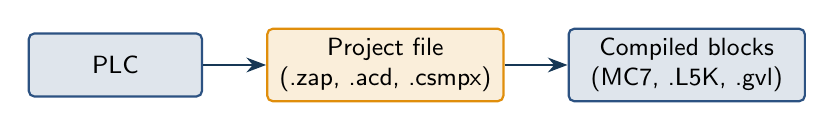
\begin{tikzpicture}[node distance=8mm]
  \node[plc, minimum width=22mm] (plc) {PLC};
  \node[isbox, fill=isAccent!15, draw=isAccent, right=of plc, minimum width=30mm, font=\small] (prj) {Project file\\(.zap, .acd, .csmpx)};
  \node[isbox, fill=isPLC!15, draw=isPLC, right=of prj, minimum width=30mm, font=\small] (rt) {Compiled blocks\\(MC7, .L5K, .gvl)};
  \draw[flow] (plc) -- (prj); \draw[flow] (prj) -- (rt);
\end{tikzpicture}
\vspace{2mm}
\begin{importantbox}{The blind spot}
The PLC runs the \emph{compiled} blocks. The vendor tool shows the \emph{project}. If an attacker changes only the runtime, the project still looks fine and only RE catches it.
\end{importantbox}
\source{Stuxnet (2010) is the canonical example -- HMI fed clean data while the PLC ran tampered logic.}
\end{frame}

\begin{frame}{Three Common Vendor Worlds}
\centering
\renewcommand{\arraystretch}{1.3}
\footnotesize
\setlength{\tabcolsep}{3pt}
\begin{tabular}{|p{2.6cm}|p{3.2cm}|p{3.4cm}|p{3.0cm}|}
\hline
\rowcolor{slidePanel}
 & \textbf{Siemens S7-3xx/4xx} & \textbf{Rockwell ControlLogix} & \textbf{CODESYS family} \\
\hline
Project file & \texttt{.zap}, \texttt{.s7p} (Step7); \texttt{.ap16} (TIA) & \texttt{.acd} & \texttt{.project} (XML zip) \\
On-PLC format & MC7 byte-code, OBxx/FCxx/DBxx blocks & \texttt{.L5K} compiled tags & UDFB structured text \\
Read-back tool & \texttt{snap7}, TIA upload & RSLogix5000 upload, \texttt{libplctag} & CODESYS device tree \\
\hline
\end{tabular}
\source{Snap7 docs; \emph{libplctag}; Rockwell PCDC; CODESYS GmbH.}
\end{frame}

\section{Acquisition}

\begin{frame}[fragile]{Reading Blocks via Snap7 (Siemens)}
\begin{lstlisting}[language=Python]
import snap7
c = snap7.client.Client()
c.connect("10.0.0.10", 0, 1)
# List blocks, then upload OB1 + DB1
blocks = c.list_blocks()                # SfcCount, OBCount, FCCount...
ob1 = c.upload(snap7.types.Block.OB, 1) # raw MC7 bytes
db1 = c.upload(snap7.types.Block.DB, 1)
open("ob1.bin", "wb").write(ob1)
\end{lstlisting}
\vspace{1mm}
\begin{notebox}{Permission check}
The S7-300/400 default \emph{put/get} setting allows upload; modern S7-1500 requires explicit enable. Document any change.
\end{notebox}
\end{frame}

\begin{frame}{Project-File Acquisition}
\centering
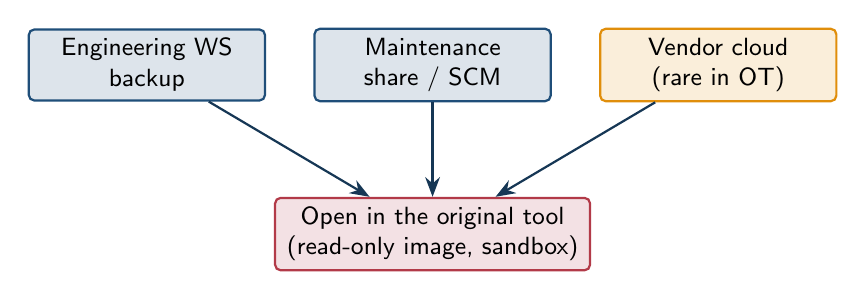
\begin{tikzpicture}[node distance=6mm]
  \node[isbox, fill=isOT!15, draw=isOT, minimum width=30mm, font=\small] (a) {Engineering WS\\backup};
  \node[isbox, fill=isOT!15, draw=isOT, right=of a, minimum width=30mm, font=\small] (b) {Maintenance\\share / SCM};
  \node[isbox, fill=isAccent!15, draw=isAccent, right=of b, minimum width=30mm, font=\small] (c) {Vendor cloud\\(rare in OT)};
  \node[isbox, fill=isAttack!15, draw=isAttack, below=12mm of b, minimum width=40mm, font=\small, align=center] (d) {Open in the original tool\\(read-only image, sandbox)};
  \draw[flow] (a) -- (d); \draw[flow] (b) -- (d); \draw[flow] (c) -- (d);
\end{tikzpicture}
\vspace{2mm}
\begin{tipbox}{Always sandbox}
Project files have run macros and \emph{network ranges}. Open them in a disconnected VM with no host shares.
\end{tipbox}
\end{frame}

\section{Decoding}

\begin{frame}{Siemens MC7 Block Layout}
\centering
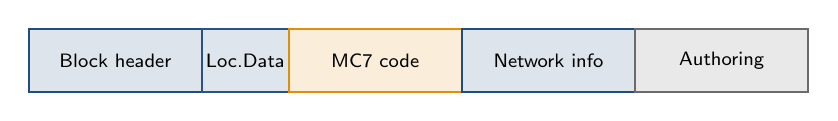
\begin{tikzpicture}[x=11mm, y=8mm, font=\scriptsize]
  \foreach \x/\w/\name/\col in {0/2/{Block header}/isOT, 2/1/{Loc.Data}/isPLC, 3/2/{MC7 code}/isAccent, 5/2/{Network info}/isOT, 7/2/{Authoring}/isMute}{
    \draw[fill=\col!15, draw=\col, thick] (\x,0) rectangle ++(\w,1);
    \node[align=center] at (\x+\w/2, 0.5) {\name};
  }
\end{tikzpicture}
\vspace{2mm}
\begin{notebox}{Tools}
\texttt{s7-pcap} and \texttt{step7-parser} (Sergey Gordeychik et al., 2015) parse MC7. Newer S7commPlus blocks (S7-1200/1500) use \texttt{Pdata} and require S7commPlus-aware tools.
\end{notebox}
\source{Sergey Gordeychik et al., \emph{SCADA StrangeLove}, 2015 \textbar{} Beresford, D., \emph{Exploiting Siemens Simatic S7 PLCs}, 2011.}
\end{frame}

\begin{frame}{Rockwell .L5K and .ACD}
\begin{itemize}
  \item \texttt{.acd} is a binary container; \texttt{.l5k} / \texttt{.l5x} is the printable export.
  \item \texttt{l5k\_parser} (community) reconstructs Structured Text from the export.
  \item Watch for \textbf{add-on instructions (AOIs)} -- compiled inside the project; their internals are hidden in the GUI.
  \item Tag aliases obscure semantics: \texttt{Bool15} may secretly be ``open\_valve''.
\end{itemize}
\begin{tipbox}{Decompile then re-render}
Round-trip the export through RSLogix; what visually matches the original is faithful, what diverges is your target.
\end{tipbox}
\end{frame}

\begin{frame}{CODESYS / IEC 61131-3 Round-Trip}
\centering
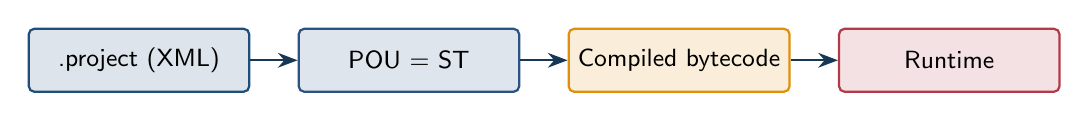
\begin{tikzpicture}[node distance=6mm]
  \node[isbox, fill=isOT!15, draw=isOT, minimum width=28mm, font=\small] (a) {.project (XML)};
  \node[isbox, fill=isPLC!15, draw=isPLC, right=of a, minimum width=28mm, font=\small] (b) {POU = ST};
  \node[isbox, fill=isAccent!15, draw=isAccent, right=of b, minimum width=28mm, font=\small] (c) {Compiled bytecode};
  \node[isbox, fill=isAttack!15, draw=isAttack, right=of c, minimum width=28mm, font=\small] (d) {Runtime};
  \foreach \s/\e in {a/b, b/c, c/d}{\draw[flow] (\s) -- (\e);}
\end{tikzpicture}
\vspace{2mm}
\begin{importantbox}{CODE16 (2023)}
Sixteen CVEs in CODESYS Runtime exposed authentication, parser, and update-verifier flaws across hundreds of vendor products built on the runtime.
\end{importantbox}
\source{CISA \emph{ICSA-23-103-09} and related advisories; Microsoft \emph{CoDe16} disclosure, 2023.}
\end{frame}

\section{What to Look For}

\begin{frame}{The Stuxnet Pattern}
\centering
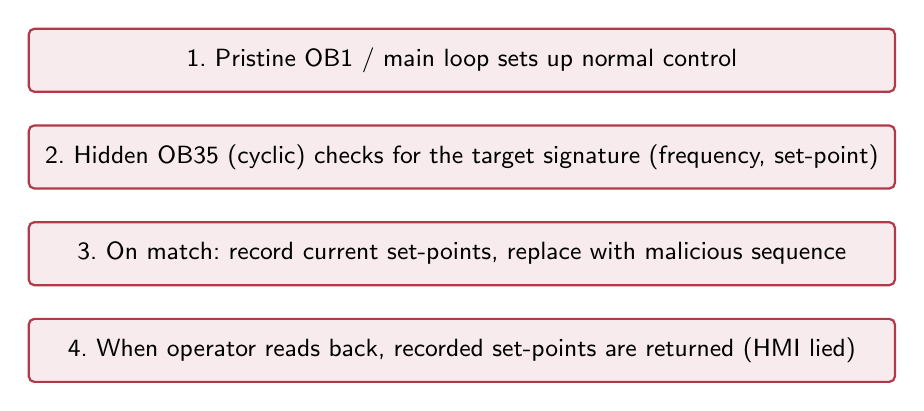
\begin{tikzpicture}[node distance=4mm]
  \node[isbox, fill=isAttack!10, draw=isAttack, minimum width=110mm, font=\small] (a) {1.\ Pristine OB1 / main loop sets up normal control};
  \node[isbox, fill=isAttack!10, draw=isAttack, minimum width=110mm, font=\small, below=of a] (b) {2.\ Hidden OB35 (cyclic) checks for the target signature (frequency, set-point)};
  \node[isbox, fill=isAttack!10, draw=isAttack, minimum width=110mm, font=\small, below=of b] (c) {3.\ On match: record current set-points, replace with malicious sequence};
  \node[isbox, fill=isAttack!10, draw=isAttack, minimum width=110mm, font=\small, below=of c] (d) {4.\ When operator reads back, recorded set-points are returned (HMI lied)};
\end{tikzpicture}
\source{Langner, R., \emph{To Kill a Centrifuge}, The Langner Group, 2013.}
\end{frame}

\begin{frame}{Logic Bomb Indicators}
\begin{itemize}
  \item Unused inputs that are read but never appear in the rung logic.
  \item Time- or counter-based branches that never fire under normal data.
  \item Blocks named after vendor utilities (``OEM\_diag'', ``factory\_test'') outside the official block list.
  \item Constants whose values match \emph{exactly} known process set-points.
  \item Calls into reserved or vendor-locked memory areas.
  \item Discrepancy between project-file timestamps and on-PLC block CRCs.
\end{itemize}
\begin{warnbox}
A missing CRC, or a CRC that does not match the project file, is more often vendor sloppiness than malice -- but it deserves a written investigation.
\end{warnbox}
\end{frame}

\begin{frame}{Tagging the Memory Map}
\centering
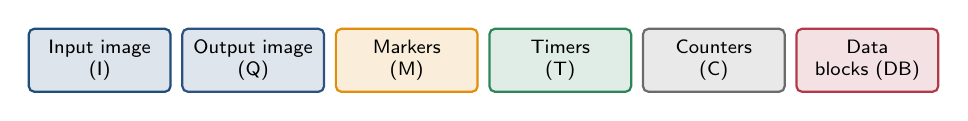
\begin{tikzpicture}[x=1.3cm, y=1cm]
  \node[isbox, fill=isOT!15, draw=isOT, minimum width=18mm, font=\scriptsize, align=center] at (0,0) {Input image\\(I)};
  \node[isbox, fill=isPLC!15, draw=isPLC, minimum width=18mm, font=\scriptsize, align=center] at (1.5,0) {Output image\\(Q)};
  \node[isbox, fill=isAccent!15, draw=isAccent, minimum width=18mm, font=\scriptsize, align=center] at (3.0,0) {Markers\\(M)};
  \node[isbox, fill=isHMI!15, draw=isHMI, minimum width=18mm, font=\scriptsize, align=center] at (4.5,0) {Timers\\(T)};
  \node[isbox, fill=isMute!15, draw=isMute, minimum width=18mm, font=\scriptsize, align=center] at (6.0,0) {Counters\\(C)};
  \node[isbox, fill=isAttack!15, draw=isAttack, minimum width=18mm, font=\scriptsize, align=center] at (7.5,0) {Data\\blocks (DB)};
\end{tikzpicture}
\vspace{2mm}
\begin{notebox}{Reverse engineering tip}
Cross-reference \emph{every} symbol against where it is read and where it is written. Symbols that are only \emph{written} (never read) are smoke.
\end{notebox}
\end{frame}

\section{Defending the Code}

\begin{frame}{Defensive Controls}
\centering
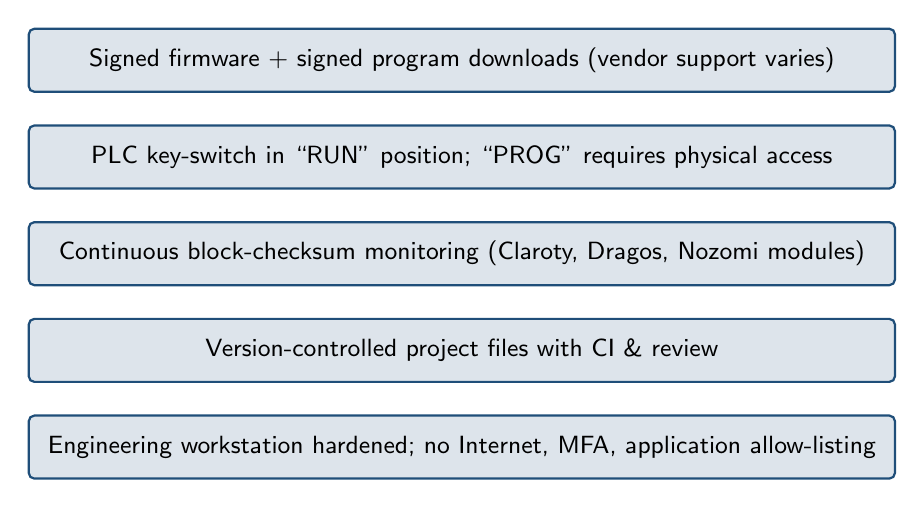
\begin{tikzpicture}[node distance=4mm]
  \node[isbox, fill=isOT!15, draw=isOT, minimum width=110mm, font=\small] (a) {Signed firmware + signed program downloads (vendor support varies)};
  \node[isbox, fill=isOT!15, draw=isOT, minimum width=110mm, font=\small, below=of a] (b) {PLC key-switch in ``RUN'' position; ``PROG'' requires physical access};
  \node[isbox, fill=isOT!15, draw=isOT, minimum width=110mm, font=\small, below=of b] (c) {Continuous block-checksum monitoring (Claroty, Dragos, Nozomi modules)};
  \node[isbox, fill=isOT!15, draw=isOT, minimum width=110mm, font=\small, below=of c] (d) {Version-controlled project files with CI \& review};
  \node[isbox, fill=isOT!15, draw=isOT, minimum width=110mm, font=\small, below=of d] (e) {Engineering workstation hardened; no Internet, MFA, application allow-listing};
\end{tikzpicture}
\end{frame}

\begin{frame}{Disclosure Considerations}
\begin{itemize}
  \item Findings on production logic touch \textbf{safety} -- coordinate with process safety, not just IT.
  \item Vendor PSIRT first; CERT/CC second; public publication only after fix.
  \item Sharing tags or constants from real plants risks identifying the asset owner -- redact heavily.
  \item Some jurisdictions (US DMCA \S1201, EU CRA research safe-harbour, German \S202c StGB) constrain RE; consult counsel.
\end{itemize}
\begin{warnbox}
Logic from a production PLC you do not own is contaminated evidence. No serious vendor will accept it.
\end{warnbox}
\end{frame}

\begin{frame}{Summary -- Section \sectionNumber}
\begin{takeawaybox}{Ladder RE for ICS}
\begin{itemize}\setlength{\itemsep}{2pt}
  \item PLCs run compiled blocks, not the project source -- they can diverge silently.
  \item Project-file and runtime acquisition each catch different attacks.
  \item Vendor-specific tools (snap7, l5k-parser, CODESYS) are the workhorses.
  \item Stuxnet-style logic bombs hide in unused inputs, time bombs, and CRC mismatches.
  \item Defence is signed downloads, key-switch, continuous checksum monitoring.
\end{itemize}
\end{takeawaybox}
\end{frame}

\referencesframe{
  \item Langner, R. \emph{To Kill a Centrifuge}, The Langner Group, Nov 2013.
  \item Falliere, N., Murchu, L., Chien, E. \emph{W32.Stuxnet Dossier}, v1.4, Symantec, 2011.
  \item Beresford, D. \emph{Exploiting Siemens Simatic S7 PLCs}, BlackHat USA, 2011.
  \item Gordeychik, S. et al. \emph{SCADA StrangeLove} talks and tools, 2014--2018.
  \item Snap7 project. \url{https://snap7.sourceforge.net}.
  \item OpenPLC project. \url{https://openplcproject.com}.
  \item ODVA. \emph{libplctag / CIP open libraries}.
  \item Rockwell Automation. \emph{Logix5000 Controllers Import/Export}, manual 1756-RM084.
  \item CISA \emph{ICSA-23-103-09} and related CODESYS advisories (CoDe16), 2023.
  \item Microsoft Threat Intelligence. \emph{CoDe16: 16 vulnerabilities in CODESYS Runtime}, 2023.
  \item IEC 61131-3:2013. \emph{Programmable controllers -- Part 3: Programming languages}.
  \item Dragos, Claroty, Nozomi. PLC integrity-monitoring product documentation.
}

\closingframe

\end{document}
